\documentclass[a4paper,11pt]{article}
\usepackage[a4paper,
            inner=30mm,
            outer=30mm,% = marginparsep + marginparwidth 
                       %   + 5mm (between marginpar and page border)
            top=20mm,
            bottom=25mm,
            marginparsep=5mm,
            marginparwidth=40mm,
            %showframe% for show your page design, normaly not used
            ]{geometry}
% PACKAGES AND MARGINS:
\usepackage[english]{babel}
\usepackage[]{units}
\usepackage{csquotes}
\usepackage{rotating}
\usepackage{tikz}
\usepackage[titletoc,title]{appendix}
\usepackage[scientific-notation=true]{siunitx}
\sisetup{round-mode=places,round-precision=1}
\def\appendixautorefname{Appendix}
\MakeOuterQuote{"}
\usepackage[breaklinks,colorlinks,citecolor=blue,linkcolor=blue]{hyperref}
\renewcommand*{\sectionautorefname}{Section}
\providecommand{\e}[1]{\ensuremath{\times 10^{#1}}}
%\usepackage[all]{hypcap}
%\usepackage[margin=0.9in]{geometry}
%\usepackage{geometry}
 %\geometry{a4paper,total={210mm,297mm},left=20mm,right=20mm,top=25mm,bottom=20m} 
\usepackage[round]{natbib}   % omit 'round' option if you prefer square brackets
%\bibliographystyle{plainnat}
%\bibliographystyle{plain}
\usepackage{graphicx}
\usepackage{subfig}
\usepackage{titling} % Set position and space of title
\linespread{1.2}
\setlength{\droptitle}{-10em}   % This is your set screw

\title{Reducing AEGIS galaxies in two filters \\
LSST DESC Note yy}
\author{Sowmya Kamath, Joshua Meyers, Patricia Burchat}
\date{\today}
\vspace{-2cm}

\begin{document}

\maketitle

\begin{abstract}
This research note summarizes the procedure used to process AEGIS HST images in V and I bands to produce multi-band postage stamp images of galaxies
\end{abstract}

\section{Introduction}
Gravitational weak-lensing is a useful tool in cosmology and requires statistical precision and accuracy in galaxy shape measurements. The chromatic nature of the point spread function (PSF) and the varying Spectral Energy Distribution (SED) across a galaxy profile can create additional complications in measuring the intrinsic shape of the observed galaxy. Hence to better understand chromatic effects on galaxy shapes measured by LSST, it is necessary to simulate galaxy images that reflect the chromatic components of real galaxies rather than only parametric models. 

We can use real galaxy images observed by HST in multiple filters to simulate real chromatic galaxies as seen by LSST, as implemented by Josh Meyers as {\tt ChromaticRealGalaxies} in {\tt GalSim} (see Github
\href{https://github.com/GalSim-developers/GalSim/issues/640}{issue}, 
\href{https://github.com/GalSim-developers/GalSim/pull/687}{pull request},
and 
\href{https://github.com/GalSim-developers/GalSim/blob/\%23640/devel/modules/CGNotes.pdf}{note}). 
In this document, we describe the procedure used to obtain postage-stamp images of individual galaxies from 
\href{http://aegis.ucolick.org/tech_overview.html}{AEGIS} 
(All-sky Extended Groth strip International Survey) in two HST filters (V and I). The method used to reduce the images is similar to the method used  to reduce COSMOS images \citep{Leauthaud2007}, and is an extension of work done by Bradley Emi, Rachel Mandelbaum, Andres Plaza, and Jason Rhodes in 2015 
(\href{https://github.com/bradleyemi/ChromaticGalaxies}{ChromaticGalaxies Github}). The final products are similar to the COSMOS Real Galaxy training sample used in the third GRavitational lEnsing Accuracy Testing challenge, or GREAT3 \citep{Mandelbaum2014}. The \href{https://github.com/sowmyakth/true_gal_colors}{script} developed for image reduction is explained in a \href{https://github.com/GalSim-developers/GalSim/blob/\%23770/devel/external/AEGIS/README.md}{README} file\footnote{https://github.com/GalSim-developers/GalSim/blob/\%23770/devel/external/AEGIS/README.md}.

The work is presented as follows. In \autoref{sec:data set} we discuss the AEGIS HST data set used as input. The image reduction procedure is described in \autoref{sec:procedure}. The resulting two-band galaxy catalog and images are described in \autoref{sec:data} and analyzed in \autoref{sec:analysis}. 

\section{Input Data Set}
We use unrotated ACS/WFC data, that was already reduced, to create the catalog. To model the PSF, we use star fields drawn from {\tt Tiny Tim} software.  
\label{sec:data set}
\subsection{AEGIS HST data}
For the AEGIS HST imaging, a mosaic pattern consisting of $21 \times 3 = 63$ contiguous HST "tiles" was used to cover an effective area of $∼10.1'\times 70.5' = 710.9$ arcmin$^2$. Each tile was observed in a 4-pointing dither pattern in each of two filters (V and I), in order to achieve half-pixel dithering at the center of the ACS WFC, bridge the detector gap, and improve tile overlap. For each of the 63 tiles, there is a science image and a weight map \citep{Davis2006}.

\subsection{Science Image and Weight Map}
Each reduced image has been drizzled from 4 exposures to produce final $8000 \times 8000$ pixel images with pixel sampling of $0.03''$ per pixel~\citep{Lotz2008}. The total exposure times and ABMAG zero-points  are shown in \autoref{table:bandpass}.

%----------------------------------
\begin{table}[htb]
\centering
\caption{Parameters for images in V and I bands.}
\label{table:bandpass}
\begin{tabular}{cccc}
\hline
\hline
Filter & Total exposure time & ABMAG zero-point  \\
\hline
 F606W (V)  &  2260\,s  & 26.508  \\
 F814W (I)  &  2100\,s  & 25.955  \\
\end{tabular}
\end{table}
%----------------------------------

The dithered observations for each pointing and filter were combined ("drizzled") using 
\href{http://stsdas.stsci.edu/multidrizzle}{MultiDrizzle}. 
The pixel drop size was 0.8 of the input pixel size, and the 
final pixel size of $0.03''$ is 0.6 of the input pixel size of $0.05''$.
These pixel sizes have been shown to reduce stochastic aliasing of the PSF~\citep{Rhodes}. 
An impact of the smaller pixel scale is increased correlation in the background noise in the final drizzled image. 
The MultiDrizzle algorithm also produces inverse-variance ($1/{\rm RMS}^2$) weight maps for each drizzled image. The weight maps include the effects of non-uniform exposure times for the "gaps" between the ACS chips and for masked cosmic-rays. The weight maps were converted to RMS maps ($\rm \sqrt[2]{\rm 1/WEIGHT\_MAP}$) for SExtractor measurements (see Appendix \autoref{App:weight} for details).

\subsection{{\tt Tiny Tim} Star Field}
The variation in the size and ellipticity of the PSF across the focal plane of the HST ACS is dominated by the effective focus, which changes due to thermal expansion and contraction of the HST. The {\tt Tiny Tim} ray-tracing software simulates the variation of the PSF across the field for different focal lengths. The PSF variation across an image is characterized by comparing the measured PSF ellipticity for stars in a field to the {\tt Tiny Tim} predictions for different focus offsets, and finding the focus that best matches the measured and predicted PSFs across the field~\citep{Leauthaud2007}.

\section{Catalog Construction Procedure}
\label{sec:procedure}
The procedure used to create the catalog is similar to that used for the weak lensing catalog for the HST ACS COSMOS survey~\citep{Leauthaud2007}. 
We use version 2.8.6 of the \href{http://www.astromatic.net/software/sextractor}{SExtractor} package to produce a source catalog of positions and various photometric parameters. The steps in the construction of the catalog and the number of objects relevant to each step are summarized in \autoref{table:count_all} and described in the following subsections.
%----------------------------------
\begin{table}[htb]
\centering
\caption{Summary of steps in construction of catalog.}
\label{table:count_all}
\resizebox{\textwidth}{!}{\begin{tabular}{lcc}
\hline
\hline
Parameter & V band & I band \\
\hline
 \multicolumn{3}{c}{Raw SExtractor Detections on Co-added V+I Image}\\
 \hline
 Total number of detected objects  & \multicolumn{2}{c} {\num{165419}} \\
 Total number of faint detections  & 
 \multicolumn{2}{c} {\num{147344}}\\
 Total number of bright detections  &  \multicolumn{2}{c} {\num{18075}}  \\
\hline
 \multicolumn{3}{c}{Details of Cleaning Process}\\
 \hline
 Number of objects within noisy border of tile  & 
 \multicolumn{2}{c} {\num{8944}}\\
 Number of faint detections with central pixel in bright segmentation map  & 
 \multicolumn{2}{c}{\num{19651}} \\
 Number of objects in diffraction masks  &  \num{1644}  & \num{1610}\\
 Number of objects in manual masks  &
 \multicolumn{2}{c}{\num{819}}\\
 Number of objects detected more than once in adjacent tiles  &
 \multicolumn{2}{c}{\num{2479}}\\
\hline
  \multicolumn{3}{c}{Catalog Cleaned of Image Defects}\\
 \hline
 Total number of objects  &  \num{134568}  & \num{134604}\\
 Number of galaxies  &  \num{133222}  & \num{132829}\\
 Number of stars  &  \num{1346}  & \num{1775}\\
\hline
 \multicolumn{3}{c}{Catalog with $\rm F814W_{AB}<25.2$}\\
 \hline
 Total number of galaxies &  
 \multicolumn{2}{c} {\num{28532}}\\
\hline
 \multicolumn{3}{c}{Final Catalog after removing bad postage stamps }\\
 \hline
Total number of galaxies  &   \multicolumn{2}{c}{\num{26517}}\\
 \hline
 \hline
\end{tabular}}
\end{table}
%----------------------------------

\subsection{Detection in Co-added Images}
We use SExtractor in dual-image mode, detecting objects with the summed V+I images and then performing photometry on the individual V and I images. This ensures that the catalogs have the same objects in both bands. 

The input RMS map corresponding to the co-added image was created by taking the reciprocal of the weight maps in both bands, adding them and then taking the square root of the content of each pixel.

\subsection{"Hot-Cold" Detection Method}
To construct a catalog of objects useful for weak-lensing studies, 
we must be efficient in detecting the small faint objects that contain much of the lensing signal. 
We therefore configure SExtractor with very low detection thresholds (even if this leads to false detections) and apply selection criteria to clean the catalog later. 
However, when configured with low detection thresholds, SExtractor inevitably deblends low surface brightness spirals and patchy irregulars, detects spurious objects in the scattered light around bright objects, and under-deblends overlapping pairs of objects. To remedy these problems we adopt the method used by ~\cite{Leauthaud2007}, which was an improvement upon the "Hot-Cold" method used in the GEMS survey data analysis ~\citep{Rix}. We run SExtractor twice, once with a configuration optimized for the detection of only the brightest objects ("cold"), and then again with a configuration optimized for the faint objects ("hot" step). The higher detection threshold of the bright step improves the detection of close pairs. Masks are created to remove false detections around bright objects, and then the two samples are merged to form the final catalog.

The Sextractor configuration parameters used for the detection of bright and faint objects are shown in \autoref{table:s_param}. 
All other parameters are set to their default values. We will refer to the resultant catalogs of detected objects as $\rm C_{bright}$ and $\rm C_{faint}$. The segementation maps created in each step are saved, to be used later when the two catalogs are merged, as well as in creating a combined segmentation map. 

%----------------------------------
\begin{table}[htb]
\centering
\caption{SExtractor configuration parameters for bright and faint object detection.}
\label{table:s_param}
\begin{tabular}{lll}
\hline
\hline
Parameter & Bright Objects  & Faint Objects  \\
\hline
DETECT\_MINAREA  &  140  & 18  \\
DETECT\_THRESH   &  2.2  & 1.0  \\
DEBLEND\_NTHRESH &  64   & 64 \\
DEBLEND\_MINCONT &  0.04 & 0.065\\
CLEAN\_PARAM     &  1.0  & 1.0 \\
BACK\_SIZE       &  400  & 100 \\
BACK\_FILTERSIZE &  5    & 3\\
BACKPHOTO\_TYPE  &  Local & Local\\
BACKPHOTO\_THICK &  200   & 200\\
\end{tabular}
\end{table}
%----------------------------------

\subsection{Merging Bright and Faint Catalogs}
\label{ssec:merge}
To remove spurious detections around bright objects, the region associated with each object in the segmentation map for the bright-object detections is extended by 15 pixels in all directions\footnote{For the COSMOS catalog of~\cite{Leauthaud2007}, a 20-pixel buffer was used around bright objects. We found that the narrower buffer remedied problems in a later step in which we combine segmentation maps; see \autoref{ssec:com_seg}.}; 
objects in the faint catalog ($\rm C_{faint}$) are then removed if their centroid lies within the extended region associated with a bright object.  
The final catalog is obtained by merging {\em all} objects in the bright catalog ($\rm C_{bright}$) with the remaining faint objects.

\subsection{Cleaning}
Care is taken to remove unreliable regions of images and false detections. 
The following regions were masked and objects detected within the regions were excluded from the final catalog.
\begin{itemize}
\item \textbf{Image boundaries}: Each ACS/WFC pointing consists of four slightly offset, dithered exposures, making detection less reliable near the boundaries of each tile where there are fewer than four input exposures. Because adjacent tiles overlap sufficiently, we are able to eliminate these regions near the boundaries without reducing the number of detected objects. 
Objects are included in the catalog only if their centroid lies within the area demarcated by the green box shown in the image on the right of \autoref{fig:mask}. The same area is used for all tiles and for both filters.
\item \textbf{Diffraction spikes}: Objects near bright stars or saturated pixels were masked to avoid shape biases due to any background gradient. Stars with magnitude less than 19 are taken to be saturated. An automatic algorithm was developed to define polygonal-shaped masks around saturated stars, with a size scaled by the FLUX\_AUTO of the star. The diffraction spike mask for a saturated star is shown as the yellow polygon in the image on the right in \autoref{fig:mask}. 
The width of the spike mask was set to 40 pixels. The length of the spike to be masked was determined with parameters from a linear fit that was made to FLUX\_AUTO versus the length of the spike measured manually, for 10 saturated stars. The angle was set to the mean of the angles by which the manually measured spikes were found to be rotated relative to the $x$-$y$ axes. The parameters defining the mask were computed separately for each filter.

%----------------------------------
\begin{figure}[th]
  \centering
  \subfloat[Raw image.]{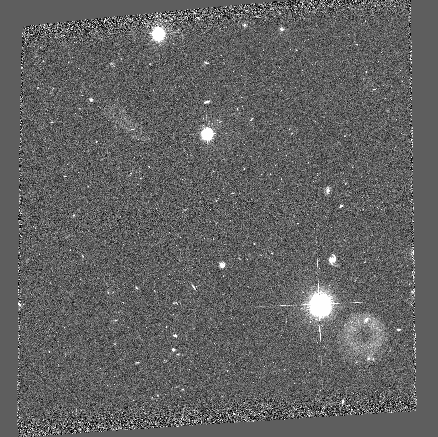
\includegraphics[width=0.5\textwidth]{im.png}}
  \hfill
  \subfloat[Boundary edge (green), automated diffraction spike mask (yellow), and manual mask (pink).]{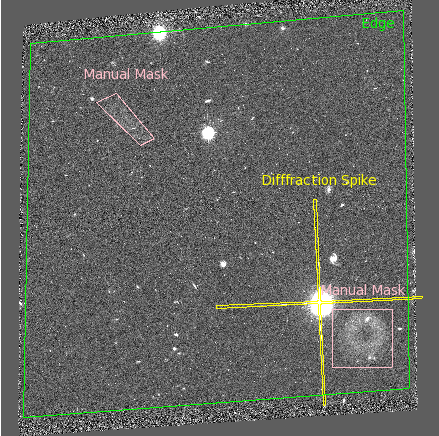
\includegraphics[width=0.5\textwidth]{im_with_mask.png}}
\caption{(a) Raw image. (b) Examples of masking.}
  \label{fig:mask}
\end{figure}
%----------------------------------
\item \textbf{Manual masks}: In a few cases where the automatic diffraction-spike masking algorithm failed, the masks were corrected by hand. Other artifacts or contaminated regions were masked, including ``ghosts'' due to internal reflections. The pink boxes in the image on the right in \autoref{fig:mask} show two such regions that were discovered upon visual inspection and manually masked.
\item \textbf{Multiple detections}: Pairs of objects whose centroids are within 2 arcseconds of each other (typically due to the overlap between adjacent tiles) were marked as multiple detections. 
The object with the highest value of SExtractor FLAG (indicating a poor detection) was discarded;
if the the multiple detections have the same FLAG, the object with  higher SNR is kept.
\end{itemize}
This gives a catalog of around \num{134568} unique detections (see \autoref{table:count_all}). 

\subsection{Star-Galaxy Separation}
Since the goal here is to obtain a sample of \textbf{galaxy} images in multiple bands, star-galaxy separation is important. Also, a clean sample of stars is important for modeling the PSF. 
The CLASS\_STAR parameter of SExtractor is unreliable since it was trained with ground-based images and is therefore only valid for a sample of profiles similar to the original training set ~\citep{Leauthaud2007}. Therefore, we use an  alternate method that was used in the COSMOS catalog construction to classify point sources and galaxies, based on the SExtractor parameters MU\_MAX (peak surface brightness above the background level) and MAG\_AUTO. 
Since the surface brightness of a point source scales with magnitude, and that of extended objects does not, stars occupy a well-defined locus in a plot of MU\_MAX vs.\,MAG\_AUTO, whereas galaxies do not.
The criteria used to classify stars and galaxies is illustrated by the black line in the plot for each filter in  \autoref{fig:star_gal}. 
Since point sources are difficult to separate from small faint galaxies, we only use star candidates with magnitudes less than 25. In the figure, the red dots denote star candidates and the blue dots galaxy candidates; stars with yellow circles are selected for PSF estimation as described below.

%---------------------------------
\begin{figure}[h]
\centering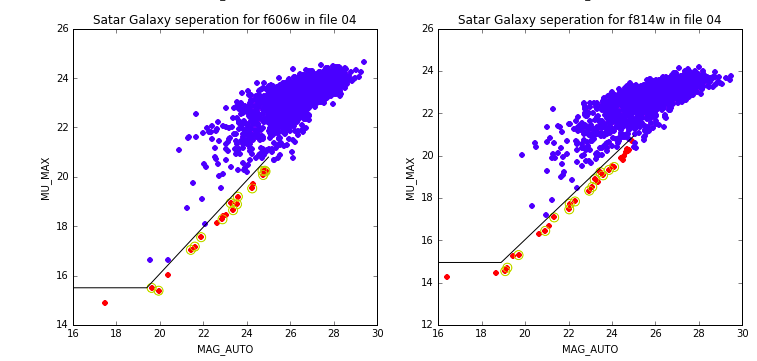
\includegraphics[width=1.\linewidth]{star_gal_04.png}
\caption{Star-galaxy separation in a plot of surface brightness vs.\,magnitude, for V band (left) and I band (right) for a single tile. 
The black line shows the line used to separate stars and galaxies.
Faint objects with magnitude above 25 are not classified as stars due to contamination from galaxies.
The red dots denote star candidates while the blue dots denote galaxy candidates.  
Stars with yellow circles are selected for PSF estimation.}
\label{fig:star_gal}
\end{figure}
%----------------------------------

\subsection{PSF Estimation}
\label{ssec:psf}
Although the ACS/WFC PSF is not stable, most of the PSF variation can be ascribed to a single physical parameter. Thermal expansions and contractions of HST alter the distance between the primary and secondary mirrors. As the effective focus deviates from nominal, the PSF becomes larger and more elliptical, with the direction of elongation depending on the position above or below nominal focus. The {\tt Tiny Tim} ray-tracing program is used to create a grid of model PSF images at varying focus offsets \citep{Rhodes}. By comparing the ellipticity of $\approx 15$ stars in each image to the {\tt Tiny Tim} predictions for those locations, we determine the image's effective focus. 

The stars for PSF estimation were selected from the up-to-25 stars with highest SNR in each image. The "star" in the {\tt Tiny Tim} model closest to each of the above stars was identified. Only star candidates that were 1) not masked, 2) had no other object close to them, 3) had a {\tt Tiny Tim} star within 200 pixels, and 4) were classified as stars in both bands were selected for PSF estimation. A cost function was defined as the sum of the squares of the differences in each ellipticity component for the real and simulated stars, where the ellipticity was defined in terms of the second moments. 
The focus offset was chosen as the one with the lowest cost function. 
A sample plot of cost function versus focus offset is shown in \autoref{fig:cf_foc}. 
The vertical dashed line shows the value of focus offset corresponding to the minimum cost function.

%---------------------------------
\begin{figure}[h]
\centering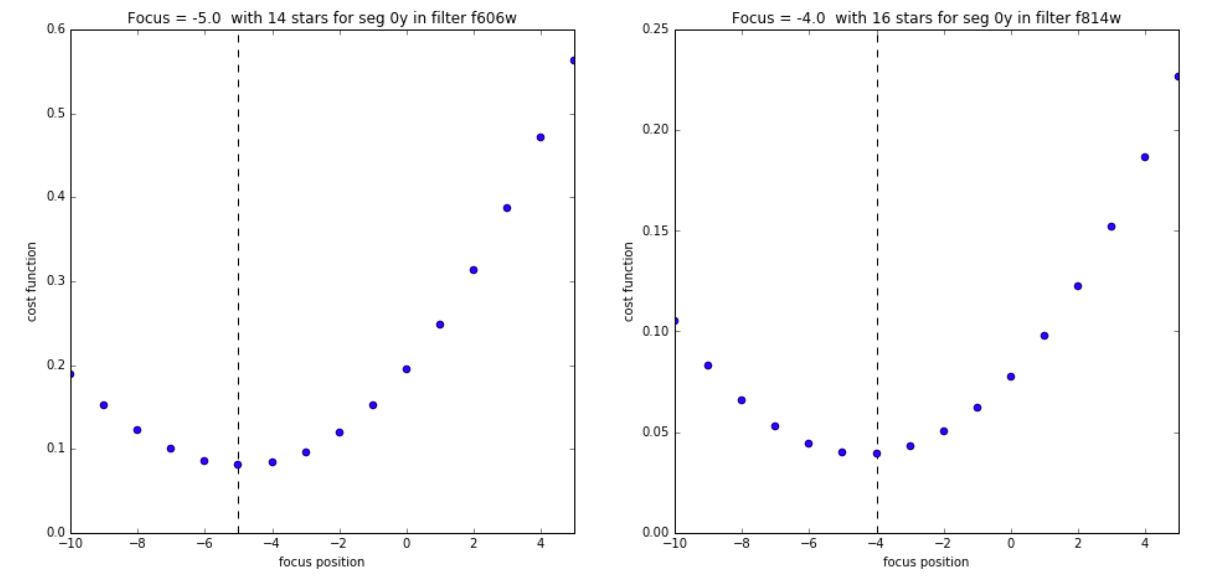
\includegraphics[width=0.8\linewidth]{cf_foc_04.png}
\caption{Cost function for different values of focus offset for V band (left) and I band (right). The vertical dashed line shows the selected focus offset value.}
\label{fig:cf_foc}
\end{figure}
%----------------------------------

For each image, the focus offset was calculated for all stars that passed the criteria described above, and then recalculated dropping the lowest SNR star. 
This was repeated until only 3 stars were left.
\autoref{fig:foc_num} shows the focus offset corresponding to the minimum value of the cost function for different numbers of stars used to compute the cost function, in a single sample image. 
The modal value of focus offset was selected for each image, illustrated with the horizontal dashed line in the image.
%---------------------------------
\begin{figure}[h]
\centering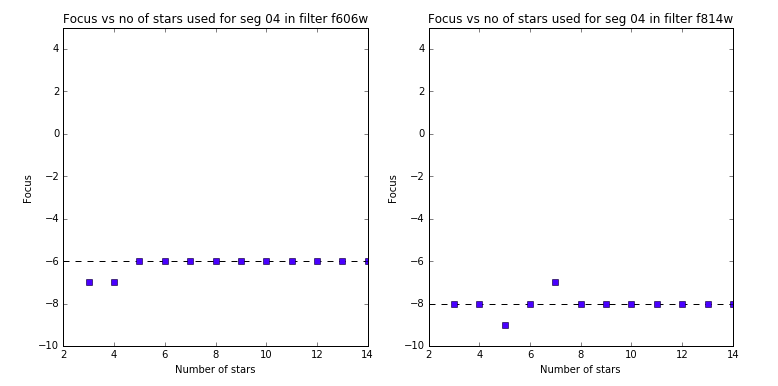
\includegraphics[width=0.8\linewidth]{foc_num_04.png}
\caption{Focus offset corresponding to minimum cost function for different numbers of stars used to calculate the cost function for V band (left) and I band (right).
The horizontal dashed line shows the focus offset selected.}
\label{fig:foc_num}
\end{figure}
%----------------------------------

\subsection{Combined Segmentation Map}
\label{ssec:com_seg}
Our main objective here is to obtain \textbf{individual} galaxy images in multiple bands -- i.e. individual postage stamps of galaxies. If there is more than one galaxy in a postage stamp, the cleaning step masks the non-central galaxies with noise. However postage stamps where the masked object is too close to the central object, or where the masking was insufficient, are identified and eliminated in the selection step.  Identifying these multiple galaxies is done with a segmentation map that includes all objects in the bright-faint merged catalog, hereafter called the combined segmentation map. Since we care more about obtaining a pure sample than a complete sample, the cleaning step has been made stringent. Eliminating a few good galaxies in the selection step is preferable to having postage stamps with multiple objects that cannot be cleaned.
There are several factors to be considered in making the combined segmentation map:
\begin{enumerate}
\item Every object in the catalog must have only one region. 
\item The detection limits and hence segmentation maps for bright and faint detections will be different. 
\item The combined map must not shred objects. 
\item Close-by objects should be identified as different regions.
\end{enumerate}

Bright/faint objects in the combined segmentation map will have a region corresponding to their region in the bright/faint segmentation map. If a pixel was detected to belong to different objects in the bright and faint step, it is assigned to the bright object. The original segmentation region corresponding to any object in the bright catalog is expanded by 5 pixels. This is done because detection limits were set much higher for the bright objects and the segmentation maps obtained thus do not encompass the whole object. 

As noted earlier (in \autoref{ssec:merge}), in the COSMOS reduction procedure, objects in the faint catalog are added to the merged catalog only if the center of the faint object does not lie inside the bright segment buffered by 20 pixels. Thus a small faint object that lies within this buffered region will not be included in the merged catalog and in the combined segmentation map; hence, it will not be replaced by noise in the cleaning step. This is why we decided to reduce the buffer size to 15 pixels. 

\subsection{Galaxy Selection}
\label{sec:gal_selection}
The following criteria are used to  select objects for the final catalog of galaxies and the corresponding set of postage stamps:
\begin{itemize}
\item The object is not classified as a star in either filter.
\item The object is not in a masked region in either filter.
\item The object has SNR $>0$ in both filters.
\item Object has MAG\_AUTO less than $25.2$ in the I (F814W) band. 
\end{itemize}

28,532 objects satisfy the above criteria (see \autoref{table:count_all}).

\subsection{Galaxy Postage Stamps}
%Only objects that satisfy the above criteria appear in the final catalog and have corresponding postage stamps. 
Rectangular postage stamps are made for each selected galaxy. 
The size of the postage stamp for each galaxy is
determined using equations 2 and 3 in \cite{Haussler2007}:
\begin{eqnarray}
{\rm XSIZE} & = 2.5\, a \, {\rm kron}\,\Big( |\sin\theta| + (1-{\rm ellip})|\cos\theta|\Big),\\
{\rm YSIZE} & = 2.5\, a \, {\rm kron}\,\Big( |\cos\theta| + (1-{\rm ellip})|\sin\theta|\Big),
\end{eqnarray}
where $a$ is the SExtractor output parameter A\_IMAGE, kron is KRON\_RADIUS, $\theta$ is THETA\_IMAGE, and ellip is ELLIPTICITY. 
The parameters XSIZE and YSIZE are individually computed for each filter and the highest value sets that dimension of the postage stamp for both filters.  
Postage stamps with the same dimensions are also drawn for the combined segmentation map and used in the cleaning step below.


\subsection{Cleaning Postage Stamps}
\label{sec:cleanpostagestamps}
In crowded regions, the galaxy postage stamp may contain other neighboring objects. These contaminating galaxies will influence shape measurements of the central galaxy and hence have to be masked. 
We ensure that there is only one galaxy per postage stamp by replacing the pixel content for the other objects with noise. 

The combined segmentation-map of the region is used to determine which pixels correspond to the central galaxy, which to the contaminating galaxies, and which are background. Pixels that correspond to any object except the central object in the galaxy postage stamp are replaced with noise drawn from a noise map created for each filter, described in \autoref{sec:noise_map} below. Thus each postage stamp has just the central galaxy image.

%----------------------------------

\subsection{Identifying Bad Postage Stamps}
\label{sec:rem_bad_stamps}

After the above cleaning step, we find that sometimes the other object is too close to the central galaxy or too bright for it to be effectively masked.
If a galaxy is too bright, then its segmentation region (computed with bright SExtractor settings)  is not able to encapsulate all the bright pixels, leading to imperfect masking. Also  if two galaxies are close to each other, the segmentation map assigns a pixel to just one galaxy or the other, leading to sharp edges. The segmentation map assigns a pixel to a single galaxy. Thus if two galaxies are close to each other, a pixel in between them  is assigned to just one galaxy. This may result in abrupt changes in the assignment of neighboring pixels, causing sharp edges in the surface brightness profiles in the cleaned galaxy postage stamps. The postage stamp cleaning step  does not take into account blended galaxies, leading to spurious galaxy shapes. 

We use the technique used in creating the dataset for the GREAT3 challenge \citep{Mandelbaum2014} to help identify such bad postage stamps.
%(see \autoref{sec:rem_bad_stamps}), 
During the cleaning step we identify the pixel that is closest to the center of the postage stamp (i.e., the center of the selected object) {\em and} has had its value replaced by noise. 
Two parameters are measured for this pixel:
\begin{enumerate}
\item  {\tt min\_mask\_dist\_pixels}: the distance from the center of the postage stamp to the closest replaced pixel;
\item {\tt average\_mask\_adjacent\_pixel\_count}: the average flux in the $3 \times 3$ pixel region around this closest replaced pixel, before replacing with noise.
\end{enumerate}
The parameters are computed separately in each band. 

A ``bad stamp'' flag is set if
\begin{enumerate}
\item {\tt HSM} module of {\tt GalSim} was not able to compute moments and the SExtractor parameter ELLIPTICITY $\leq $ 0.75, in any filter.
\item {\tt min\_mask\_dist\_pixels} $\leq $ 5 pixels from the center
\item $5<$ {\tt min\_mask\_dist\_pixels} $\leq $ 11 pixels {\em and} {\tt average\_mask\_adjacent\_pixel\_count} is greater than 20\% of the brightest-pixel value.
\end{enumerate}
Galaxies with the bad stamp flag in any filter are removed from the final catalogs of both filters.
We are left with 26,517 good galaxy postage stamps in our final catalog, for both bands.

\subsection{Creating the Noise Map}
\label{sec:noise_map}
The drizzling process introduces correlations between neighboring pixels, which artificially reduces the noise level of co-added drizzled images. Care is taken to preserve these correlations when generating noise maps to replace pixel values for nearby objects. 
 
Sixteen empty regions of varying sizes, with dimensions ranging from 70-700 pixels,  at different positions on the image plane, were visually identified. A $50\times50$ covariance matrix for the pixel values was calculated for each empty region (separately in each filter) and their mean computed, as shown in \autoref{fig:covar}.
Noise maps generated from the mean covariance matrix for each filter are shown in \autoref{fig:noise_map}.

%----------------------------------
\begin{figure}[h]
  \centering
  \subfloat[Covariance map in V (F606W) filter.]{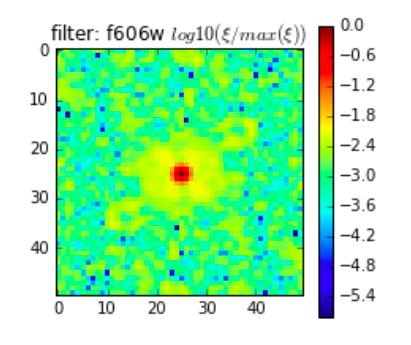
\includegraphics[width=0.4\textwidth]{covar_f814.png}}
  \hfill
  \subfloat[Covariance map in I (F814W) filter.]{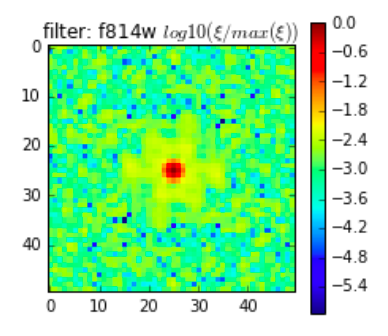
\includegraphics[width=0.4\textwidth]{covar_f606.png}}
  \caption{Mean co-variance matrix in the two filters.}
  \label{fig:covar}
\end{figure}
%----------------------------------

%---------------------------------
\begin{figure}[h]
\centering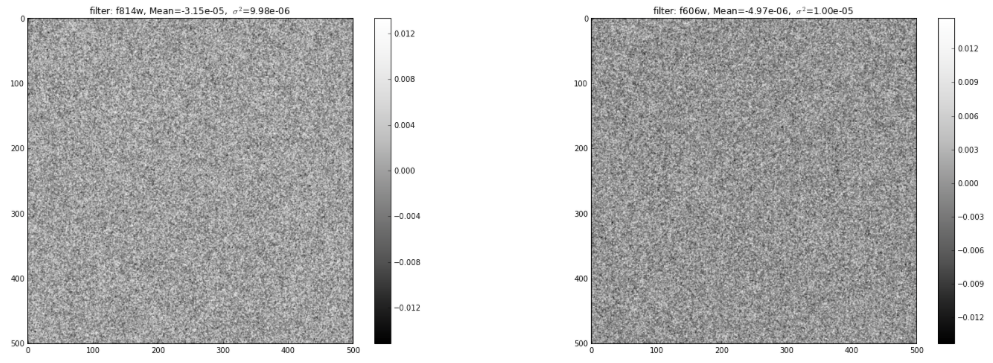
\includegraphics[width=1.\linewidth]{noise_map.png}
\caption{Image of noise map generated from covariance matrices, for I band (left) and V band (right).}
\label{fig:noise_map}
\end{figure}
%----------------------------------

To replace nearby objects with noise, a region that is identical in size and shape to the nearby object in the segmentation map is cut from a random location in the noise map shown in \autoref{fig:noise_map} and used to replace the pixel values for the nearby object in the galaxy postage stamp.  

\subsection{Parametric Fits}
The COSMOS catalog galaxies for the GREAT3 challenge were subject to an additional step of fitting for parametric models. This step was not performed here, and the values in the output catalogs corresponding to these parameters were manually set to 999.

\subsection{PSF Postage Stamp}
The PSF for each galaxy is taken to be the {\tt Tiny Tim} model PSF image whose location in the {\tt Tiny Tim} grid is closest to that galaxy's position in the focal plane, for the best-fit focus offset described in \autoref{ssec:psf}. Square postage stamps ($20 \times 20$ pixels) are drawn for each filter.

\subsection{Additional Catalogs}
The Extended Groth Strip (EGS) has been extensively studied with other surveys in other bands. 
We include in our catalog photometry and spectroscopic redshift measurements from other catalogs, for objects in our catalog with a center within $1''$ of an object in the other catalog.

We include in our final catalog the spectroscopic redshifts for 3763 matched galaxies from the DEEP2 galaxy redshift survey, Data Release 4 \citep{Newman2013}. 
The redshift distribution for these matched galaxies is shown in \autoref{fig:redshift}. 

%---------------------------------
\begin{figure}[h]
\centering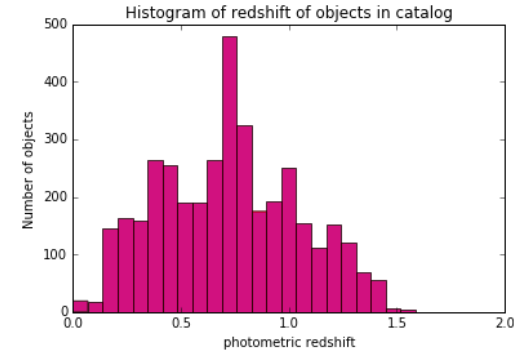
\includegraphics[width=0.7\linewidth]{redshift.png}
\caption{Spectroscopic redshifts for selected galaxies that also appear in the DEEP2 redshift survey.}
\label{fig:redshift}
\end{figure}
%----------------------------------
We also include in our catalog the results from the photometry catalog of the AEGIS field~\citep{Lotz2008}. 
We compare in \autoref{fig:cat_mag} the magnitude we measure with SExtractor to the magnitude in the AEGIS photometry catalog for 27,289 matched objects. The magnitudes of bright objects in the two catalogs are in good agreement. However  for larger magnitudes, there are a few objects that are measured to be fainter in the AEGIS photometric catalog than in this catalog.
%---------------------------------
\begin{figure}[h]
\centering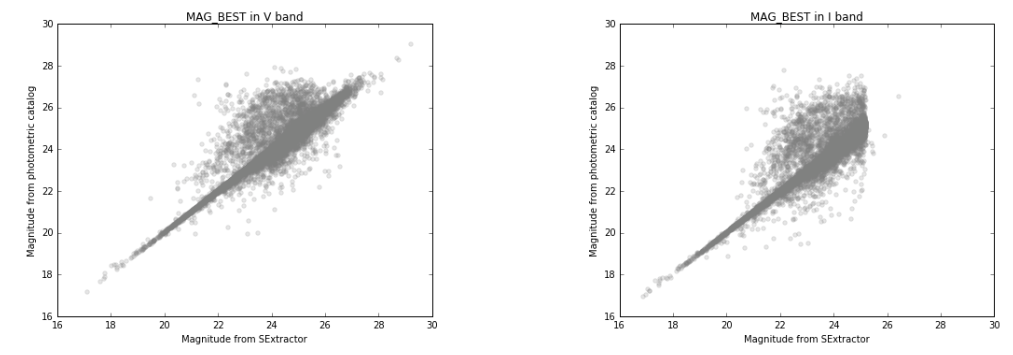
\includegraphics[width=1.\linewidth]{cat_mag.png}
\caption{Magnitudes in AEGIS catalog plotted versus magnitudes calculated with SExtractor for this study.}
\label{fig:cat_mag}
\end{figure}
%----------------------------------
\section{Data Products}
\label{sec:data}
The output files are in the format expected by {\tt galsim.RealGalaxyCatalog}. The format of the output files and the saved attributes are explained in detail in the AEGIS catalog  \href{https://github.com/sowmyakth/true_gal_colors/blob/master/AEGIS_25.2_training_sample_readme.txt}{README} file. 
For each band, there are several output files:
\begin{enumerate}
\item Main catalog (hereafter referred to as the GalSim catalog);
\item Files with postage stamp images of galaxies;
\item Files with postage stamp images of PSF;
\item Catalog with information on parametric fits (step not performed here);
\item Catalog with information for selection cuts;
\item File with noise correlation function.
\end{enumerate}

The GalSim catalogs contain only select details about the galaxies. A complete catalog with more columns is also created which has all the columns in the GalSim catalog, parametric fits catalog, selection catalog, information from additional catalogs and other measured values from SExtractor. 

\section{Object Characteristics}
\label{sec:analysis} 
In \autoref{fig:mag_all}, we show the distribution of magnitudes computed by SExtractor in V and I band, and V$-$I color, as well as a color-magnitude plot, for the 26,517 objects in the final catalog. 
Recall from \autoref{sec:gal_selection} that a magnitude cut of 25.2 was made in the I band only.
%---------------------------------
\begin{figure}[h]
\centering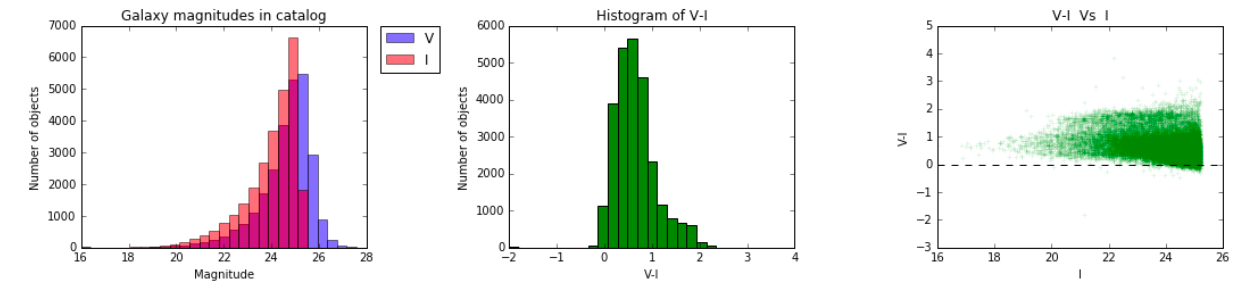
\includegraphics[width=1.\linewidth]{AEGIS_magnitude.png}
\caption{Distributions for the 29,105 selected objects. a) Magnitude in V band and I band. b) Difference in magnitudes (V$-$I color).  c) V$-$I color vs.~I band magnitude.}
\label{fig:mag_all}
\end{figure}
%----------------------------------

In \autoref{fig:sn_ellip}, we show the SNR distribution in each band for the selected galaxies. 
The SNR was measured with an elliptical Gaussian filter matched to the galaxy profile with the {\tt HSM} module of {\tt GalSim}. 
This SNR calculation does not take into account the fact that the noise is correlated between pixels; hence the noise is under-estimated.  
The corrected SNR would be approximately half the values plotted here (see section 3.8 in \cite{Leauthaud2007}).

%---------------------------------
\begin{figure}[h]
\centering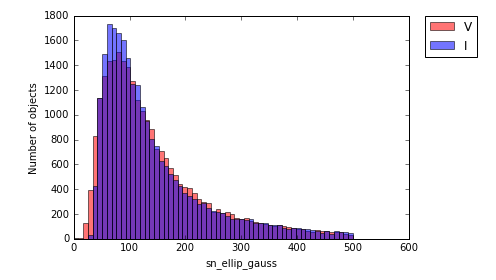
\includegraphics[width=0.9\linewidth]{sn_ellip_all.png}
\caption{Distribution of the galaxy flux SNR,  measured with an elliptical Gaussian filter.}
\label{fig:sn_ellip}
\end{figure}
%----------------------------------

In \autoref{fig:pstamps}, postage stamps are shown for the galaxy images (left) and the corresponding {\tt Tiny Tim} PSF images (right) for V band (top) and I band (bottom), for a sample galaxy. 
As noted in earlier sections, the size of the galaxy postage stamp is the same for the two filters, and the PSF postage stamps are always 20 pixel $\times$ 20 pixel squares. 

%---------------------------------
\begin{figure}[h]
\centering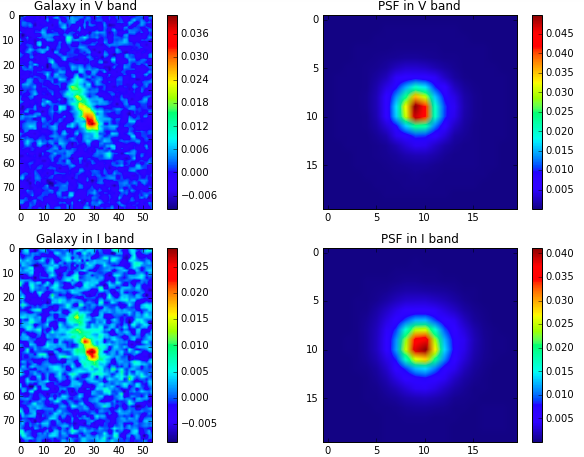
\includegraphics[width=1.\linewidth]{pstamps.png}
\caption{Postage stamps for the galaxy images (left) and the corresponding {\tt Tiny Tim} PSF images (right) for V band (top) and I band (bottom), for a sample galaxy.}
\label{fig:pstamps}
\end{figure}
%----------------------------------

\subsection{Selection Effects and Weight Function}

%---------------------------------
\begin{figure}[h]
\centering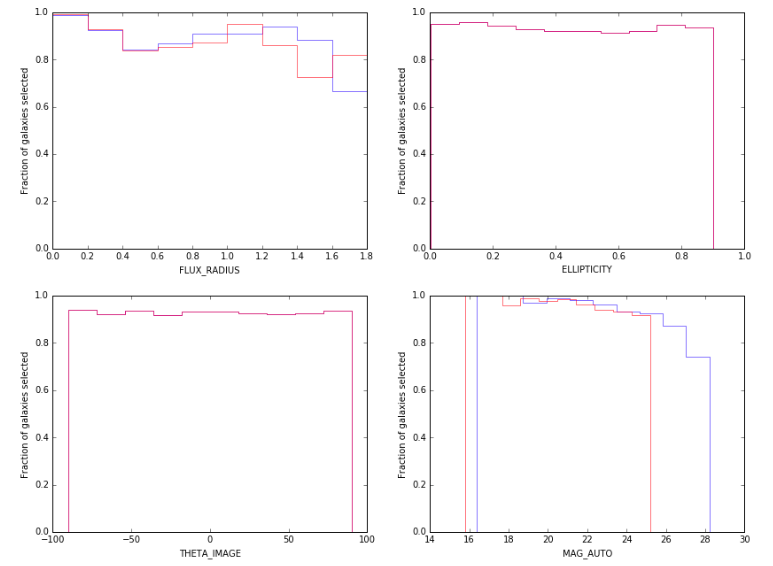
\includegraphics[width=0.8\linewidth]{frac_param.png}
\caption{Histogram of fraction of galaxies selected in the final catalog as a function of half-light radius, ellipticity, position angle, and magnitude 
in I band (red) and V band (blue).}
\label{fig:frac_param}
\end{figure}
%----------------------------------

The process of picking galaxies for the final catalogs can introduce certain unwanted selection effects. 
Selection effects would be evident in plots of the fraction of initially detected galaxies  that are included in the final catalog, as a function of galaxy properties. 
% Could you specify precisely what ``initially detected'' corresponds to here? Does the initially detected sample contain objects that aren't actually galaxies -- e.g., shredded galaxies, blended galaxies, noise near bright objects,...? In other words, it is important to specify which of the selections in Table 2 are being addressed here. Which row in the table does the initial sample correspond to?}
Selection effects become evident when the galaxies that pass the selection cuts to be included in the final catalog (\num{26517} galaxies in \autoref{table:count_all}, hereafter final catalog) are compared to the galaxies in the catalog of galaxies with $\rm F814W_{AB}<25.2$ (\num{28532} galaxies in \autoref{table:count_all}, hereafter parent catalog) \autoref{fig:frac_param} shows histograms of the fraction of galaxies from the parent catalog included in the final catalog as a function of four parameters estimated by SExtractor: {\tt FLUX\_RADIUS} (half-light radius), {\tt ELLIPTICITY} (magnitude of ellipticity, $1-b/a$), {\tt THETA\_IMAGE} (position angle) and {\tt MAG\_AUTO} (AB magnitude). We can see a clear dependence of the fraction on the size of the galaxy, while the other parameters don't seem to influence it. 
%It looks like there is a significant dependence on magnitude. Is this correlated with size? To check, remake the magnitude histograms with weighted entries to see if it is then flat.
A drop in the fraction of selected galaxies for large galaxies is primarily due to larger galaxies being shredded during the detection step, causing  them to be improperly masked in the postage stamp cleaning step, thereby failing the selection cuts. 

%---------------------------------
\begin{figure}[h]
\centering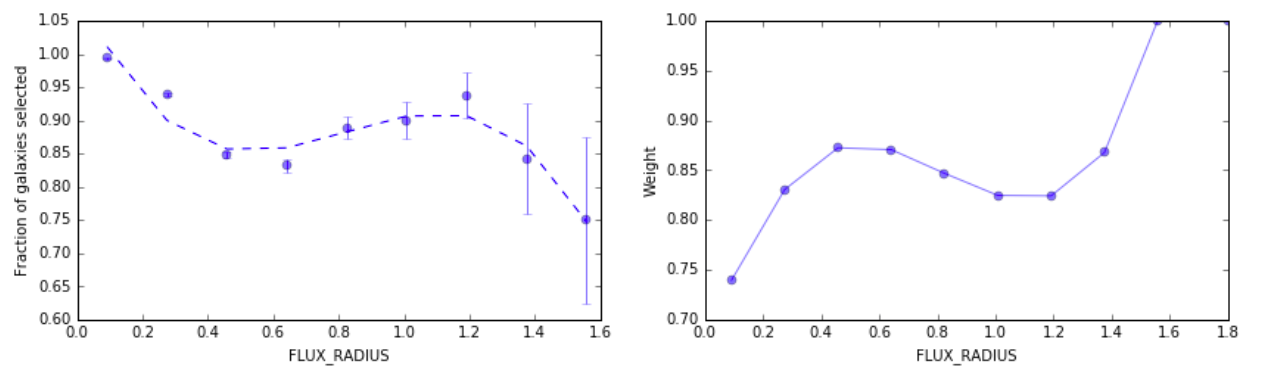
\includegraphics[width=1.\linewidth]{frac_weight.png}
\caption{Left: Fraction of galaxies selected in the final catalog as a function of half-light-radius (solid dots) along with the fitted curve (dashed line). Right: Weights computed for different half-light-radii. The weight is defined such that large galaxies have value 1.}
\label{fig:frac_weight}
\end{figure}
%----------------------------------

%---------------------------------
\begin{figure}[h]
\centering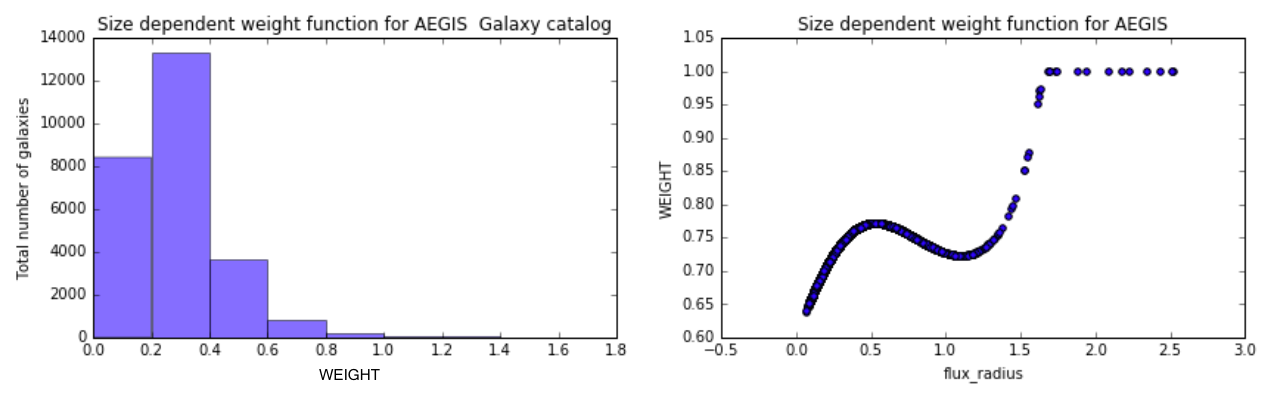
\includegraphics[width=1.\linewidth]{hist_weight.png}
\caption{Left: Histogram of weights of all the galaxies in the final catalog. 
Right: Weights of all the galaxies as function of half-light-radius.
}
\label{fig:hist_weight}
\end{figure}
%----------------------------------

To account for this selection bias we assign a size-dependent weight to every galaxy. Since the magnitude cut was applied only to the I band, the weight is computed only in this band. Thus galaxies in both bands have the same {\tt WEIGHT}, computed based on its I-band size. The weight is defined as the reciprocal of the fraction of galaxies that passed the selection cuts, normalized to 1 for large galaxies. The left panel of \autoref{fig:frac_weight} shows the fraction as a function of half-light radius (solid points). A curve is fit through the points (dashed line) and used to compute the weight for different galaxy sizes. The right panel shows the computed weight as a function of half-light-radius. A histogram of weights (left) and their distribution with size (right) for the entire final catalog is shown in \autoref{fig:hist_weight}


\section{Future Work}
This work was done with the intention of obtaining real galaxy images in the two AEGIS HST bands to produce realistic chromatic galaxy images as would be seen by other surveys. However, the pipeline can be used to reduce any HST images in multiple bands -- e.g., the CANDELS survey. Parametric fits can be performed on the galaxies and studied. The images can also be used for the analysis of multi-band galaxy fits.

%\bibliographystyle{astroads.bst}
\bibliographystyle{apj.bst}
\bibliography{AEGIS}
%----------------------------------
%APPENDIX
\newpage
\begin{appendices}
\section{Weight Maps as Input to SExtractor} \label{App:weight}
SExtractor handles images with variable noise through weight maps, which describe the expected noise level at each pixel. These maps are internally stored in units of absolute variance (in ADU$^2$). Several types of weight maps can be input to SExtractor, which converts the map to its internal variance format, controlled through the WEIGHT\_TYPE configuration keyword. If a variance map is given as input -- i.e., WEIGHT\_TYPE is MAP\_VAR -- then the input file is assumed to contain a weight map in units of {\em relative} variance. A robust scaling to the appropriate {\em absolute} variance is then performed by comparing this variance map to an internal, low-resolution, absolute variance map built from the science image itself. 
If WEIGHT\_TYPE is MAP\_WEIGHT, then the specified FITS image must contain a weight map in units of relative weights (proportional to the inverse of the variance). The data are converted to variance units ($\propto$ 1/weight) and scaled as for MAP\_VAR. 
Finally, if WEIGHT\_TYPE is MAP\_RMS, then the input map must be in units of absolute standard deviations (in ADUs per pixel). (See Section 8 in the  \href{http://www.astromatic.net/pubsvn/software/sextractor/trunk/doc/sextractor.pdf}{SExtractor manual} for details.)

Now the AEGIS weight map from MultiDrizzle is produced with weight type MAP\_WEIGHT, but with {\em absolute} units. Since  SExtractor assumes MAP\_WEIGHT (and MAP\_VAR) weight types to be in {\em relative units}, 
we save the square root of the reciprocal of each weight map pixel in a new weight map and set the weight type to MAP\_RMS so that 
no normalization is performed by SExtractor. 
\end{appendices}
\end{document}
